\documentclass[10pt,a4paper]{article}
\usepackage[top = 1.6cm, left = 3cm, right = 3cm ]{geometry}
\usepackage[utf8]{inputenc}
\usepackage[francais]{babel}
\usepackage[T1]{fontenc}
\usepackage{lmodern}
\usepackage{amsmath}
\usepackage{amsfonts}
\usepackage{amssymb}
\usepackage{graphicx}
\usepackage{float}
\usepackage{longtable}
\usepackage{hyperref}
\begin{document}
\begin{titlepage}

\newcommand{\HRule}{\rule{\linewidth}{0.5mm}} % Defines a new command for the horizontal lines, change thickness here

\center % Center everything on the page
 
%----------------------------------------------------------------------------------------
%	HEADING SECTIONS
%----------------------------------------------------------------------------------------

\textsc{\LARGE Université de Mons}\\[1.5cm] % Name of your university/college
\textsc{\Large Simulation sur ordinateur }\\[0.5cm] % Major heading such as course name

%----------------------------------------------------------------------------------------
%	TITLE SECTION
%----------------------------------------------------------------------------------------

\HRule \\[0.4cm]
{ \huge \bfseries Etude du caractère aléatoire des décimales de $\pi$}\\[0.4cm] % Title of your document
\HRule \\[1.5cm]
 
%----------------------------------------------------------------------------------------
%	AUTHOR SECTION
%----------------------------------------------------------------------------------------

\begin{minipage}{0.4\textwidth}
\begin{flushleft} \large
\emph{Auteurs :}\\
Florent Delgrange \\
Clément Tamines
\end{flushleft}
\end{minipage}
~
\begin{minipage}{0.4\textwidth}
\begin{flushright} \large
\emph{Professeur:} \\
Dr. Alain Buys
\end{flushright}
\end{minipage}\\[4cm]

% If you don't want a supervisor, uncomment the two lines below and remove the section above
%\Large \emph{Author:}\\
%John \textsc{Smith}\\[3cm] % Your name

%----------------------------------------------------------------------------------------
%	DATE SECTION
%----------------------------------------------------------------------------------------

{\large 02 juin 2016}\\[3cm] % Date, change the \today to a set date if you want to be precise

%----------------------------------------------------------------------------------------
%	LOGO SECTION
%----------------------------------------------------------------------------------------

%\includegraphics{Logo}\\[1cm] % Include a department/university logo - this will require the graphicx package
 
%----------------------------------------------------------------------------------------

\vfill % Fill the rest of the page with whitespace

\end{titlepage}

\newpage
\tableofcontents
\newpage

\section{Introduction}
	Le but de ce projet est de montrer le caractère pseudo-aléatoire des décimales de $\pi$. Nous allons montrer dans ce rapport que les 
décimales de $\pi$ suivent une distribution uniforme. Nous étudierons ce caractère pseudo-aléatoire via les tests vus au cours. Nous
créerons ensuite un générateur de nombres pseudo-aléatoires grâce aux décimales de $\pi$ fournies. Enfin, nous comparerons ce générateur
avec le générateur intégré à Python.

\section{Tests sur les décimales de $\pi$}

Nous allons maintenant étudier le caractère pseudo-aléatoire de $\pi$ grâce à plusieurs tests statistiques. \`A l'aide de séquences générées à partir de modèles faisant intervenir une loi uniforme, nous pourrons montrer le caractère pseudo-aléatoire des décimales à conditions que celles-ci aient les mêmes propriétés que les séquences.

\subsection{Test de $\chi^2$}
Le test de $\chi^2$ va nous permettre de tester l'adéquation des décimales de pi avec les familles de lois de probabilités que nous allons traiter par la suite. Pour se faire, on génère des séquences théoriques selon la loi de probabilité et on les répartis, ainsi que les décimales de $\pi$, en classes. Les effectifs de chaque classe sont comparés aux effectifs théoriques au moyen de l'équation ci-dessous :
\[ K = \displaystyle\sum_{i=1}^n (\frac{n_i-Np_i}{\sqrt{Np_i}})^2\]
où $n_i$ est l'effectif observé de la classe $i$ et $Np_i$, l'effectif théorique (loi uniforme) de la classe $i$. On soumet le test à une probabilité $\alpha$ de rejeter l'hypothèse nulle $H_0$. Celle-ci est acceptée si $K \leq \chi_x^2$ où $x$ est le degré de liberté. \\Celui-ci s'obtient facilement : $x$ = nombre de classes - 1. \\

Soit $H_0$ = \{\textit{ les décimales de $\pi$ suivent une loi uniforme }\}, considérons une classe par chiffre, on a donc que le degré de liberté est $x = 10 - 1 = 9 $. On considère donc que l'effectif d'une classe est le nombre d'occurrence de ce même digit parmi les $1e6$ décimales présentes dans le fichier fourni. On vérifie maintenant la concordance des décimales de pi avec la loi uniforme.
\begin{figure}[h!]
\makebox[\textwidth][c]{\includegraphics[width=0.7\textwidth]{khi2_histopi.png}}
\caption{Occurrence des digits de pi}
\label{khi2histo}
\end{figure}

\begin{figure}[H]
\begin{center}
\begin{longtable}{|c|c|c|}
\hline
r & eff. observé & eff. théorique\\
\hline
1 & 99959 & 100000\\
2 & 99758 & 100000\\
3 & 100026 & 100000\\
4 & 100229 & 100000\\
5 & 100230 & 100000\\
6 & 100359 & 100000\\
7 & 99548 & 100000\\
8 & 99800 & 100000\\
9 & 99985 & 100000\\
10 & 100106 & 100000\\
\hline
\end{longtable}
\end{center}
\caption{Tableau des effectifs pour chaque classe.}
\end{figure}
\begin{figure}[H]
\begin{center}
\begin{tabular}{|c|c|c|c|}
\hline
$\alpha$ & $K_{n}$ & $\chi^2_{9, 1 - \alpha}$ & Résultat\\
\hline
0.001 & 5.50908 & 27.8771648713 & True\\
0.025 & 5.50908 & 19.0227677986 & True\\
0.05 & 5.50908 & 16.9189776046 & True\\
0.1 & 5.50908 & 14.6836565733 & True\\
\hline
\end{tabular}
\end{center}
\caption{Résultat du test de $\chi^2$}
\label{result1}
\end{figure}

Les résultats obtenus nous indiquent que le test de $\chi^2$ est réussi pour tous les $\alpha$ choisis (voir figure \ref{result1}).
\subsection{Test du gap}

Le test de Gap va nous permettre de générer des classes selon une intervalle $[a, b]$ choisie préalablement. Le but est de compter les nombres compris entre 2 valeurs successives appartenant à cette intervalle, c'est ce qui représente la longueur d'un gap. Une longueur de gap correspond à une classe.\\
Afin d'adapter le test de Gap aux décimales de $\pi$, et donc à un jeu de données à valeur \textbf{discrètes}, on considère qu'une longueur de gap survient entre la récurrence d'un digit fixé au préalable.\\

Soient $u_1, u_2, u_3, ..., u_i, ..., u_{1e6}$, les décimales de $\pi$, avec $0 \leq u_i \leq 9$. Après avoir sélectionné un digit $\delta$, on va sélectionner les décimales $u_j$ telles que $u_j = \delta$. Ces $u_j$ ont une probabilité $P(x=\delta) = 0.1$. On calcule ensuite les distances entre chaque occurrence de $\delta$.\\ Soit $l_n$, la probabilité d'une longueur de gap $n$, tel que $0 \leq n \leq i$.
\[l_n = P(x \neq \delta)^n P(x=\delta)\]
\[l_i = P(x \neq \delta)^i P(x=\delta)\]
\[l_{>i} = P(x \neq \delta)^{i+1}\]
\[\Leftrightarrow l_n = 0.9^n0.1\]
\[\Leftrightarrow l_i = 0.9^i0.1\]
\[\Leftrightarrow l_{>i} = 0.9^{i+1}\]

Prenons $\delta = 5$ et $i=80$.

%---------------------------------------------------------------------
% GAP TEST
%---------------------------------------------------------------------

\begin{figure}[H]
\makebox[\textwidth][c]{\includegraphics[width=0.7\textwidth]{gap_histopi.png}}
\caption{Longueur du gap pour $\delta = 5$}
\label{khi2histo}
\end{figure}

\begin{figure}[H]
\begin{center}
\begin{longtable}{|c|c|c|}
\hline
longueur du gap & eff. observé & eff. théorique\\
\hline
0 & 10232 & 10035.9\\
1 & 8957 & 9032.31\\
2 & 8091 & 8129.079\\
3 & 7301 & 7316.1711\\
4 & 6586 & 6584.55399\\
5 & 5943 & 5926.098591\\
6 & 5392 & 5333.4887319\\
7 & 4758 & 4800.13985871\\
8 & 4364 & 4320.12587284\\
9 & 4003 & 3888.11328556\\
10 & 3530 & 3499.301957\\
$\vdots$ & $\vdots$ & $\vdots$ \\ 
50 & 51 & 51.7227726031\\
51 & 42 & 46.5504953428\\
52 & 43 & 41.8954458085\\
53 & 38 & 37.7059012277\\
54 & 33 & 33.9353111049\\
55 & 36 & 30.5417799944\\
$\vdots$ & $\vdots$ & $\vdots$ \\ 
75 & 3 & 3.71316743696\\
76 & 4 & 3.34185069327\\
77 & 1 & 3.00766562394\\
78 & 1 & 2.70689906155\\
79 & 2 & 2.43620915539\\
80 & 2 & 2.19258823985\\
81 & 23 & 19.7332941587\\
\hline
\end{longtable}
\end{center}
\caption{Tableau des effectifs pour chaque classe.}
\end{figure}
\begin{figure}[H]
\begin{center}
\begin{tabular}{|c|c|c|c|}
\hline
$\alpha$ & $K_{n}$ & $\chi^2_{81, 1 - \alpha}$ & Résultat\\
\hline
0.001 & 69.4981721617 & 126.082558333 & True\\
0.025 & 69.4981721617 & 107.783409665 & True\\
0.05 & 69.4981721617 & 103.009508712 & True\\
0.1 & 69.4981721617 & 97.6795807085 & True\\
\hline
\end{tabular}
\end{center}
\caption{Résultat du test de $\chi^2$}
\label{result2}
\end{figure}

Les résultats visibles à la figure \ref{result2} montrent que le test de $\chi^2$ effectués sur les effectifs représentant le test du gap est réussi pour tous les $\alpha$ choisis.

\subsection{Test du poker}

Le test du poker consiste en la comparaison entre le fréquences théoriques des mains au poker avec les
fréquences observées dans notre jeu de données. Pour transformer nos données en une main de poker, nous allons d'abord transformer les $1 000 000$ de décimales de $\pi$ en $200 000$ nombres de $5$ chiffres. Pour ce faire, nous allons simplement parcourir la liste des décimales fournie et y prendre 5 chiffres à la fois pour créer des nombres.\newline \newline

Nous allons ensuite compter le nombre de chiffres différents contenus dans ces nombres, ce qui nous donnera nos classes de la manière
suivante : \\
\begin{itemize}
\item Tous les chiffres sont différents
\item Deux chiffres sont identiques
\item Trois chiffres sont identiques
\item Quatre chiffres sont identiques
\item Tous les chiffres sont identiques
\end{itemize}
\bigskip
En connaissant $r$ le nombre de chiffres composant le nombre, nous pouvons calculer la probabilité $P_r$ d'une de ces configurations.
Le nombre de manières de constituer $r$ paquets avec $k$ nombres est le nombre de Stirling dont la formule est la suivante :

\begin{equation*}
\begin{Bmatrix}
k\\
r
\end{Bmatrix}
=
\begin{Bmatrix}
k-1\\
r-1
\end{Bmatrix}
+
\begin{Bmatrix}
k-1\\
r
\end{Bmatrix}
\end{equation*}
avec 
\begin{equation*}
\begin{Bmatrix}
k\\
1
\end{Bmatrix}
=
\begin{Bmatrix}
k\\
r
\end{Bmatrix}
=
1
\end{equation*}
Nous allons multiplier par le nombre de façons d'affecter les paquets aux intervalles et diviser par le nombre de façons de répartir k nombres dans les intervalles pour obtenir la probabilité.\\
\begin{equation*}
P_r = 
\frac{\begin{Bmatrix}
k\\
r
\end{Bmatrix}d(d-1) ...(d-r+1)}{d^k}
\end{equation*}
\newline
Dans notre cas nous avons des séquences de 5 chiffres ($k=5$), 10 chiffres possibles ($d=10$) et 5 classes citées précédemment ($r = 1...5$).\\
Nous allons ensuite comparer les nombres observés d'occurrences de chaque classe et les comparer avec les valeurs théoriques avec un test de $\chi^2$ . Ces nombres d'occurrences théoriques sont obtenues en multipliant la probabilité calculée par la formule précédente par le nombre d'échantillons (un nombre de 5 chiffres constitue un échantillon) sur lequel le test est effectué (dans notre cas, ce nombre est 200000). \newline

La figure \ref{pokerhisto} montre les nombres d'occurrences théoriques et les nombres d'occurences théorique. Le nombre d'occurrences de séquences ayant 5 chiffres identiques est extrêmement petit, qui explique pourquoi il n'est pas visible.\\

\begin{figure}[H]
\makebox[\textwidth][c]{\includegraphics[width=0.7\textwidth]{poker_histogram.png}}
\caption{Comparaison des résultats du test de Poker}
\label{pokerhisto}
\end{figure}

Le tableau suivant montre les valeurs obtenues pour les classes du test de Poker ainsi que le résultat du test de $\chi^2$.
\begin{figure}[H]
\begin{center}
\begin{longtable}{|c|c|c|}
\hline
Configurations & eff. observé & eff. théorique\\
\hline
Tous les chiffres identiques & 13 & 20.0\\
4 chiffres identiques & 2644 & 2700.0\\
3 chiffres identiques & 36172 & 36000.0\\
2 chiffres identiques & 100670 & 100800.0\\
Tous les chiffres différents & 60501 & 60480.0\\
\hline
\end{longtable}
\end{center}
\caption{Tableau des effectifs pour chaque classe.}
\end{figure}
\begin{figure}[H]
\begin{center}
\begin{tabular}{|c|c|c|c|}
\hline
$\alpha$ & $K_{n}$ & $\chi^2_{4, 1 - \alpha}$ & Résultat\\
\hline
0.001 & 4.60820965608 & 18.4668269529 & True\\
0.025 & 4.60820965608 & 11.1432867819 & True\\
0.05 & 4.60820965608 & 9.48772903678 & True\\
0.1 & 4.60820965608 & 7.77944033973 & True\\
\hline
\end{tabular}
\end{center}
\caption{Résultat du test de $\chi^2$}
\end{figure} 

Nous remarquons que les décimales de $\pi$ fournies réussissent le test de Poker pour tous les $\alpha$ choisis.
\subsection{Test du collectionneur de coupons}
Le test du collectionneur de coupons s'effectue en créant des séquences de chiffres à partir de la liste des décimales de $\pi$ On augmente la séquence d'un chiffre tant qu'elle ne contient pas tous les chiffres possibles. Une fois que tous les chiffres sont contenus dans la séquence, la taille de celle-ci est sauvée et devient sa classe. Une autre séquence est alors construite. Ce procédé continue tant qu'il reste des chiffres dans la liste de décimales fournie.\newline

Nous pouvons calculer le nombre théorique d'occurrences pour chaque longueur de séquence de la manière suivante :

Il est tout d'abord logique que des séquences de longueur strictement inférieure à 10 ne seront jamais observées. En effet il est impossible que tous les chiffres de 1 à 9 soient contenus dans une telle séquence. \newline
Il est possible de calculer la probabilité $S_r$ de contenir tous les chiffres dans une séquence de longueur $r$ avec la formule suivante
\begin{equation*}
S_r = 
\begin{Bmatrix}
r-1\\
d-1
\end{Bmatrix}
\frac{d!}{d^r}
\end{equation*}
Avec $r$ la taille de la séquence et $d$ le nombre de chiffres différents voulus dans celle-ci.\newline
Il est aussi possible de calculer le nombre d'occurrences pour des séquences de longueur $t>r$. La probabilité pour qu'on ait les 10 chiffres dans une séquence de taille supérieure à un certain $t$ est 

\begin{equation*}
1- 
\begin{Bmatrix}
t-1\\
d
\end{Bmatrix}
\frac{d!}{d^t-1}
\end{equation*}
Pour obtenir les nombres d'occurrences théoriques, nous avons multiplié ces probabilités par le nombre de séquences crées par le test.\newline
 
La figure \ref{couponshisto} présente les nombres d'occurrences théoriques et les nombres d'occurrences observées pour des tailles de séquence allant de 0 à 100. Nous avons remarqués que pour des tailles supérieures ou égales à 100, le nombre d'occurrence pour les différentes tailles était très petit voir nul pour certaines tailles. Nous avons alors décidés de nous limiter à des tailles strictement inférieures à 100 tout en mettant le nombre de séquences de taille supérieure ou égales à 100 dans une classe spéciale et en la comparant au nombre d'occurrence théorique calculés avec la formule présentée ci-avant. Ceci explique que les deux barres les plus à droite sur le graphique ont un nombre d'occurrences plus élevés.
\begin{figure}[H]
\makebox[\textwidth][c]{\includegraphics[width=0.7\textwidth]{coupons_histogram.png}}
\caption{Comparaison des résultats du test du collectionneur de coupons}
\label{couponshisto}
\end{figure}
Le tableau suivant présente les résultats pour le test du collectionneur de coupons : 

\begin{figure}[H]
\begin{center}
\begin{longtable}{|c|c|c|}
\hline
longueur de la sequence & eff. observé & eff. théorique\\
\hline
1 & 0 & 0 \\
2 & 0 & 0 \\
3 & 0 & 0 \\
4 & 0 & 0 \\
5 & 0 & 0 \\
6 & 0 & 0 \\
7 & 0 & 0 \\
8 & 0 & 0 \\
9 & 0 &0\\
10 & 12 & 12.39706944\\
11 & 62 & 55.78681248\\
12 & 154 & 143.186152032\\
13& 265 & 276.144721776\\
14& 496 & 445.677125782\\
15& 645 & 636.605631934\\
16& 869 & 832.196551932\\
17& 1008 & 1017.53193425\\
18& 1150 & 1181.29471772\\
19 & 1341 & 1316.26375399\\
20 & 1354 & 1418.98670105\\
$\vdots$ & $\vdots$ & $\vdots$ \\ 
90 & 0 & 2.89087837644\\
91 & 1 & 2.60186344817\\
92 & 4 & 2.34173543126\\
93 & 4 & 2.10760855074\\
94& 0 & 1.89688502594\\
95 & 1 & 1.70722638771\\
96 & 1 & 1.53652764053\\
97 & 4 & 1.38289398981\\
98 & 0 & 1.24461988155\\
99 & 2 & 1.120170126\\
100 & 12 & 9.07385754262\\
\hline
\end{longtable}
\end{center}
\caption{Tableau des effectifs pour chaque classe.}
\end{figure}

Le tableau suivant nous donne le résultat du test de $chi^2$ utilisé pour comparer nos observations avec les effectifs théoriques. Nous remarquons que le test est réussi pour tous les $\alpha$ donnés.
\begin{figure}[H]
\begin{center}
\begin{tabular}{|c|c|c|c|}
\hline
$\alpha$ & $K_{n}$ & $\chi^2_{100, 1 - \alpha}$ & Résultat\\
\hline
0.001 & 79.735983847 & 149.449252779 & True\\
0.025 & 79.735983847 & 129.561197186 & True\\
0.05 & 79.735983847 & 124.342113404 & True\\
0.1 & 79.735983847 & 118.498003811 & True\\
\hline
\end{tabular}
\end{center}
\caption{Résultat du test de $\chi^2$}
\end{figure} 

\section{Générateur de nombres pseudo-aléatoire}
Nous allons maintenant expliquer comment générer des nombres aléatoires dans $[0, 1[$ à partir des décimales de $\pi$ et cela de manière uniforme. Ensuite, nous comparerons ce générateur avec celui inclus dans Python.
\subsection{Principe}
Le moment précis auquel on demande de générer un nombre est le seul véritable caractère aléatoire que nous pourrons utiliser pour créer le générateur. On utilise donc le temps en millisecondes écoulé depuis le 1$^{er}$ janvier 1970. Afin d'obtenir dans un intervalle de temps très petit des valeurs complètement différentes, on ne retient que les 6 premiers chiffres après la virgule du nombre obtenu et on inverse l'ordre de ses chiffres (simplement via des opérations de modulo et de divisions entières). Le nombre résultant correspond à un indice dans le tableau des décimales de $\pi$. On charge de cette façon 16 indices, ce qui va correspondre à 16 digits. Ces 16 chiffres forment un nombre $x \in [0, 1e16[$. Il suffit de le diviser par $1e16$ et on obtient un nombre à 16 chiffres après la virgule dans l'intervalle $[0, 1[$. Si on veut récupérer un autre nombre aléatoire, il suffit d'ajouter 1 à tous les indices récupérés (modulo 1e6) à l'étape précédente et recommencer le processus. En résumé, on a donc 16 compteurs, qu'on itère de 1 à chaque requête de génération de nombre aléatoire, qui correspondent chacun à un indice dans le tableau des décimales de $\pi$, à partir desquels on obtient 16 digits qui forment un nombre aléatoire. Notons qu'après 1 million d'itérations, de par l'incrémentation des compteurs, des nombres précédemment générés vont apparaitre car on aura parcouru l'entièreté des décimales de $\pi$. Pour palier à cela, on réinitialise le générateur et ses compteurs à l'aide du temps UNIX.\\

Afin de comparer le générateur avec celui de Python, chacun des deux générateurs vont générer 1 million de valeurs. Nous allons appliquer les tests de la section précédente à ces deux générateurs. Ces tests ne seront plus appliqués à des valeurs discrètes, mais cette fois à des valeurs continues. On travaille cette fois avec des classes comprises dans l'intervalle $[0, 1[$. Le meilleur générateur sera celui qui aura la plus petite valeur de $K$. On se sert donc de $\chi^2$ pour vérifier lequel des deux générateurs suit le plus une loi normale et continue.

\subsection{Test de $\chi^2$}

Le test est identique à celui présenté dans la section précédente, à une exception près : les classes correspondent à des intervalles de 0.1. On génère donc 1 million de nombres.

\begin{figure}[H]
\makebox[\textwidth][c]{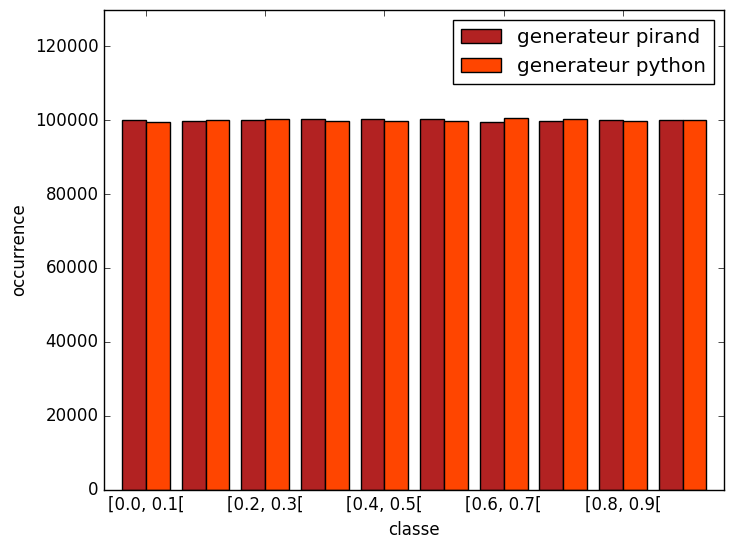
\includegraphics[width=0.7\textwidth]{comparative_histogram.png}}
\label{couponshisto}
\end{figure}

%---------------------------------------------------------------------
% KHI2 TEST
%---------------------------------------------------------------------

\begin{figure}[H]
\begin{center}
\begin{longtable}{|c|c|c|c|}
\hline
classes & eff. observé ($\pi$ rand) & eff. observé (Python rand) & eff. théorique\\
\hline
1 & 99959 & 99416 & 100000.0\\
2 & 99758 & 100078 & 100000.0\\
3 & 100026 & 100421 & 100000.0\\
4 & 100229 & 99801 & 100000.0\\
5 & 100230 & 99747 & 100000.0\\
6 & 100359 & 99750 & 100000.0\\
7 & 99548 & 100510 & 100000.0\\
8 & 99800 & 100219 & 100000.0\\
9 & 99985 & 99916 & 100000.0\\
10 & 100106 & 100142 & 100000.0\\
\hline
\end{longtable}
\end{center}
\caption{Tableau des effectifs pour chaque classe.}
\end{figure}
\begin{figure}[H]
\begin{center}
\begin{tabular}{|c|c|c|c|c|}
\hline
$\alpha$ & $K_{\pi}$ & $K_{Python}$ & $\chi^2_{9, 1 - \alpha}$ & Résultat\\
\hline
0.001 & 5.50908 & 10.25772 & 27.8771648713 & True\\
0.025 & 5.50908 & 10.25772 & 19.0227677986 & True\\
0.05 & 5.50908 & 10.25772 & 16.9189776046 & True\\
0.1 & 5.50908 & 10.25772 & 14.6836565733 & True\\
\hline
\end{tabular}
\end{center}
\caption{Résultat du test de $\chi^2$}
\end{figure}
Le générateur utilisant $\pi$ semble mieux s'en tirer que celui de Python en obtenant une valeur de $K_n$ inférieure. On peut en conclure que le générateur qui utilise $\pi$ génère des nombre de façon plus fidèle à la loi uniforme que le générateur de Python.
\subsection{Test du gap}
\'Etant donné que nous travaillons maintenant avec des valeurs continues, nous allons compter le nombre de valeurs qui ne sont pas dans l'intervalle [a, b] choisie. Nous choisissons l'intervalle $[0, 0.5]$. Nous allons donc compter le nombre de valeurs qui n'appartiennent pas à cette intervalle jusqu'à la prochaine valeur appartenant à $[0, 0.5]$, et cela pour les 1 million de valeur générées.\\

Soient $u_1, u_2, u_3, ..., u_i, ..., u_{1e6}$, les nombres générés et $0 \leq u_i < 1$. On marque les valeurs $u_j$ telles que $u_j \in [0, 0.5]$. Ces $u_j$ ont une probabilité $p = 0.5 - 0 = \frac{1}{2}$. On calcule ensuite les distances entre 2 nombres marqués.\\ Soit $l_n$, la probabilité d'une longueur de gap $n$, tel que $0 \leq n \leq i$.
\[I_0 = p = \frac{1}{2}\]
\[I_1 = (1 - p)p = \frac{1}{2} \frac{1}{2} = \frac{1}{4}\]
\[I_i = (1 - p)^ip = \frac{1}{2^i}\frac{1}{2} = \frac{1}{2^{i+1}}\]
\[I_{>i} = (1 - p)^{i + 1} = \frac{1}{2^{i+1}}\]
Prenons i = 15.\\

%---------------------------------------------------------------------
% GAP TEST
%---------------------------------------------------------------------

\begin{figure}[H]
\begin{center}
\resizebox{\columnwidth}{!}{%
\begin{tabular}{|c|c|c|c|c|}
\hline
longueur du gap & eff. observé ($\pi$ rand) & eff. observé (Python rand) & eff. théorique ($\pi$ rand) & eff. théorique (Python rand)\\
\hline
0 & 249634 & 249658 & 250101.0 & 249731.5\\
1 & 125768 & 124877 & 125050.5 & 124865.75\\
2 & 62542 & 62333 & 62525.25 & 62432.875\\
3 & 31257 & 31146 & 31262.625 & 31216.4375\\
4 & 15477 & 15672 & 15631.3125 & 15608.21875\\
5 & 7748 & 7782 & 7815.65625 & 7804.109375\\
6 & 3923 & 3945 & 3907.828125 & 3902.0546875\\
7 & 1876 & 2049 & 1953.9140625 & 1951.02734375\\
8 & 959 & 1010 & 976.95703125 & 975.513671875\\
9 & 510 & 497 & 488.478515625 & 487.756835938\\
10 & 255 & 240 & 244.239257812 & 243.878417969\\
11 & 128 & 132 & 122.119628906 & 121.939208984\\
12 & 59 & 74 & 61.0598144531 & 60.9696044922\\
13 & 28 & 29 & 30.5299072266 & 30.4848022461\\
14 & 20 & 13 & 15.2649536133 & 15.242401123\\
15 & 9 & 4 & 7.63247680664 & 7.62120056152\\
16 & 9 & 2 & 7.63247680664 & 7.62120056152\\
\hline
\end{tabular}%
}
\end{center}
\caption{Tableau des effectifs pour chaque classe.}
\end{figure}
\begin{figure}[H]
\begin{center}
\begin{tabular}{|c|c|c|c|c|}
\hline
$\alpha$ & $K_{\pi}$ & $K_{Python}$ & $\chi^2_{16, 1 - \alpha}$ & Résultat\\
\hline
0.001 & 14.5425807974 & 18.4629649622 & 39.2523547908 & True\\
0.025 & 14.5425807974 & 18.4629649622 & 28.8453507234 & True\\
0.05 & 14.5425807974 & 18.4629649622 & 26.2962276049 & True\\
0.1 & 14.5425807974 & 18.4629649622 & 23.5418289231 & True\\
\hline
\end{tabular}
\end{center}
\caption{Résultat du test de $\chi^2$}
\label{gapresult2}
\end{figure}
Encore une fois, les résultats du test de $\chi^2$ présentés à la figure \ref{gapresult2} sont meilleurs du côté du générateur utilisant $\pi$.

\subsection{Test du poker}
Afin de comparer les deux générateur en utilisant le test du poker nous allons prendre les nombres aléatoires $\in [0,1[$, les multiplier par 10 et prendre leur partie entière. Nous obtenons ainsi des nombres $\in [0,1,2,3,4,5,6,7,8,9]$. Nous pouvons ensuite effectuer le test du poker tel que décrit précédemment sur les données ainsi transformées. Effectuer le test sur ces données transformées est équivalent à diviser $[0,1]$ en 10 intervalles, car 0 correspondra à l'intervalle $[0,0.1[$ 1 à l'intervalle $[0.1,0.2[$ et ce jusqu'à 9 qui correspondra à $[0.9,1[$.\newline \newline
La figure \ref{poker_generator_histogram} présente le nombre d'occurrences théoriques et le nombre d'occurrences observées pour les deux générateurs.

\begin{figure}[H]
\makebox[\textwidth][c]{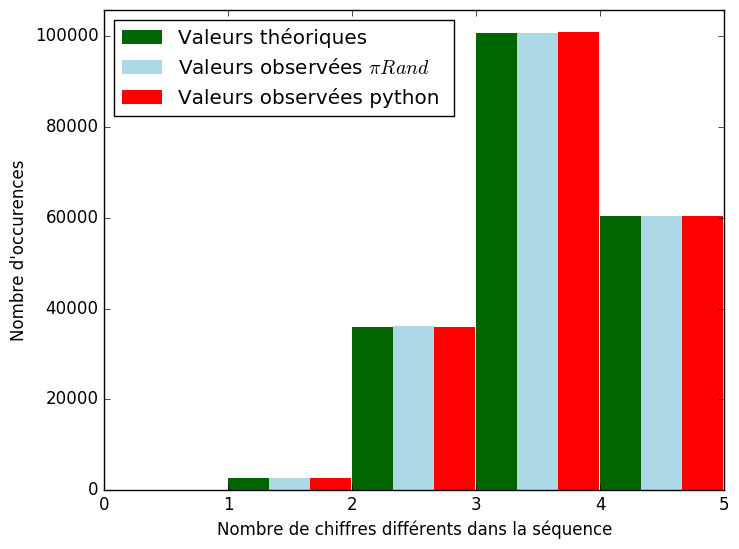
\includegraphics[width=0.7\textwidth]{poker_generator_histogram.png}}
\caption{Comparaison des générateurs pour le test du poker}
\label{poker_generator_histogram}
\end{figure}
Le tableau suivant reprend les valeur observées et les valeurs théoriques pour les deux générateurs :
\begin{figure}[H]
\begin{center}
\begin{longtable}{|c|c|c|c|c|}
\hline
classes & eff. observé ($\pi$Rand) & eff. observé (Python rand) & eff. théorique\\
\hline


Tous les chiffres identiques  & 25 & 28 & 20.0\\
4 chiffres identiques & 2721 & 2640 & 2700.0\\
3 chiffres identiques & 36136 & 36014 & 36000.0\\
2 chiffres identiques & 100678 & 100875 & 100800.0\\
Tous les chiffres différents  & 60440 & 60443 & 60480.0\\
\hline
\end{longtable}
\end{center}
\caption{Tableau des effectifs pour chaque classe.}
\end{figure}
\begin{figure}[H]
\begin{center}
\begin{tabular}{|c|c|c|c|c|}
\hline
$\alpha$ & $K_{\pi Rand}$ & $K_{Python}$ & $\chi^2_{4, 1 - \alpha}$ & Résultat\\
\hline
0.001 & 2.10122486772 & 4.61721693122 & 18.4668269529 & True\\
0.025 & 2.10122486772 & 4.61721693122 & 11.1432867819 & True\\
0.05 & 2.10122486772 & 4.61721693122 & 9.48772903678 & True\\
0.1 & 2.10122486772 & 4.61721693122 & 7.77944033973 & True\\
\hline
\end{tabular}
\end{center}
\caption{Résultat du test de $\chi^2$}
\end{figure}

Nous remarquons que le générateur de python suit mieux les effectifs théoriques pour le test du poker. Nous en concluons que le générateur de python est meilleur pour ce test.

\subsection{Test de Kolmogorov-Smirnov}
Le test de Kolmogorov-Smirnov est un test permettant de tester si les données observées sont engendrées par une loi connue. Nous devons donc connaitre cette loi et celle-ci doit être continue. Pour effectuer le test, nous allons comparer l'écart maximum entre la fonction de répartition théorique F et la fonction de répartition empirique $F_n$. Dans notre cas, F sera la loi uniforme continue.
\begin{center}
 $ F_n(x) = \frac{\text{nombre de valeurs } \leq x}{n}$\\ 
 $ F(x) =
\left\{
	\begin{array}{lll}
		0  & \mbox{si  } x < 0 \\
		x & \mbox{si  } 0 \leq x < 1 \\
		1 & \mbox{si  } x \geq 1 \\
	\end{array}
\right.
$
\end{center}
Et on va calculer $D_n = \max_{x\in R} |F_n(x)-F(x)|$ \\
Pour que le test réussisse, il faut que les valeurs de $D_n$ soient inférieurs aux valeurs théoriques $D_\alpha$ pour un $\alpha$ choisi. Le tableau suivant reprend les valeurs de $D_\alpha$ en fonction des valeurs de $\alpha$ pour des $n > 35$. 

\begin{center}
\begin{tabular}{|c|c|c|c|c|c|}
\hline
$\alpha$ &0.01& 0.05& 0.10& 0.15& 0.2\\
\hline
$D_\alpha$ & $\frac{1.63}{\sqrt{n}}$ & $\frac{1.36}{\sqrt{n}}$ & $\frac{1.22}{\sqrt{n}}$ & $\frac{1.14}{\sqrt{n}}$ & $\frac{1.07}{\sqrt{n}}$\\
\hline
\end{tabular}
\end{center}
Le tableau suivant donne les résultats du test obtenus pour les deux générateurs : \\\\
\begin{tabular}{|c|c|c|c|c|c|c|}
\hline
 $n$ & $D_{n} (pirand)$ & $D_{n} (python)$ & $\alpha$ & $D_{\alpha}$ & Res pirand & Res python\\ 
\hline 
100&0.08219&0.06524 & 0.01&0.163 & True & True\\\hline 
100&0.08219&0.06524 & 0.05&0.136 & True & True\\\hline 
100&0.08219&0.06524 & 0.1&0.122 & True & True\\\hline 
100&0.08219&0.06524 & 0.15&0.114 & True & True\\\hline 
100&0.08219&0.06524 & 0.2&0.107 & True & True\\\hline 
1000&0.03044&0.03801 & 0.01&0.05155 & True & True\\\hline 
1000&0.03044&0.03801 & 0.05&0.04301 & True & True\\\hline 
1000&0.03044&0.03801 & 0.1&0.03858 & True & True\\\hline 
1000&0.03044&0.03801 & 0.15&0.03605 & True & False\\\hline 
1000&0.03044&0.03801 & 0.2&0.03384 & True & False\\\hline 
10000&0.01442&0.00591 & 0.01&0.0163 & True & True\\\hline 
10000&0.01442&0.00591 & 0.05&0.0136 & False & True\\\hline 
10000&0.01442&0.00591 & 0.1&0.0122 & False & True\\\hline 
10000&0.01442&0.00591 & 0.15&0.0114 & False & True\\\hline 
10000&0.01442&0.00591 & 0.2&0.0107 & False & True\\\hline
\end{tabular}\\
\newline 
Nous remarquons que le générateur de python et le notre passent le test pour des séquences de 100 et 1000 nombres générés. Pour des séquences de 10000, notre teste passe seulement pour $\alpha = 0.01$. Nous pouvons en déduire que notre générateur est un peu inférieur à celui de python.


\end{document}
